% Chapter 6

\chapter[Video Tracking System]{Video Tracking System} % Main chapter title

\label{Chapter6} % For referencing the chapter elsewhere, use \ref{Chapter6} 

%----------------------------------------------------------------------------------------

In order to implement the augmented reality element of the system, and satisfy the related objectives, a live video feed of the swarm was needed. A method for tracking the positions of each individual robot in the swarm within each video frame in this feed was also required, in order to correctly position the graphical overlays. Prior to the start of this project infrastructure had been put in place at the YRL for performing this kind of video-based tracking task, in the form of a machine vision camera placed above an 'arena'. Figure \ref{fig:CameraLayout} shows the arrangement of the machine vision camera used for robot tracking, and the robot arena. Figure \ref{fig:ArenaPhoto} shows a photo of the robot arena and tracking camera set up at the YRL. Ongoing research being carried out by members of the YRL had already made use of this camera and arena set up, in conjunction with image processing software for tracking fiducial markers within the image, to achieve robot tracking with good accuracy and relatively high frame-rate.

\begin{figure}[h]
	\centering
	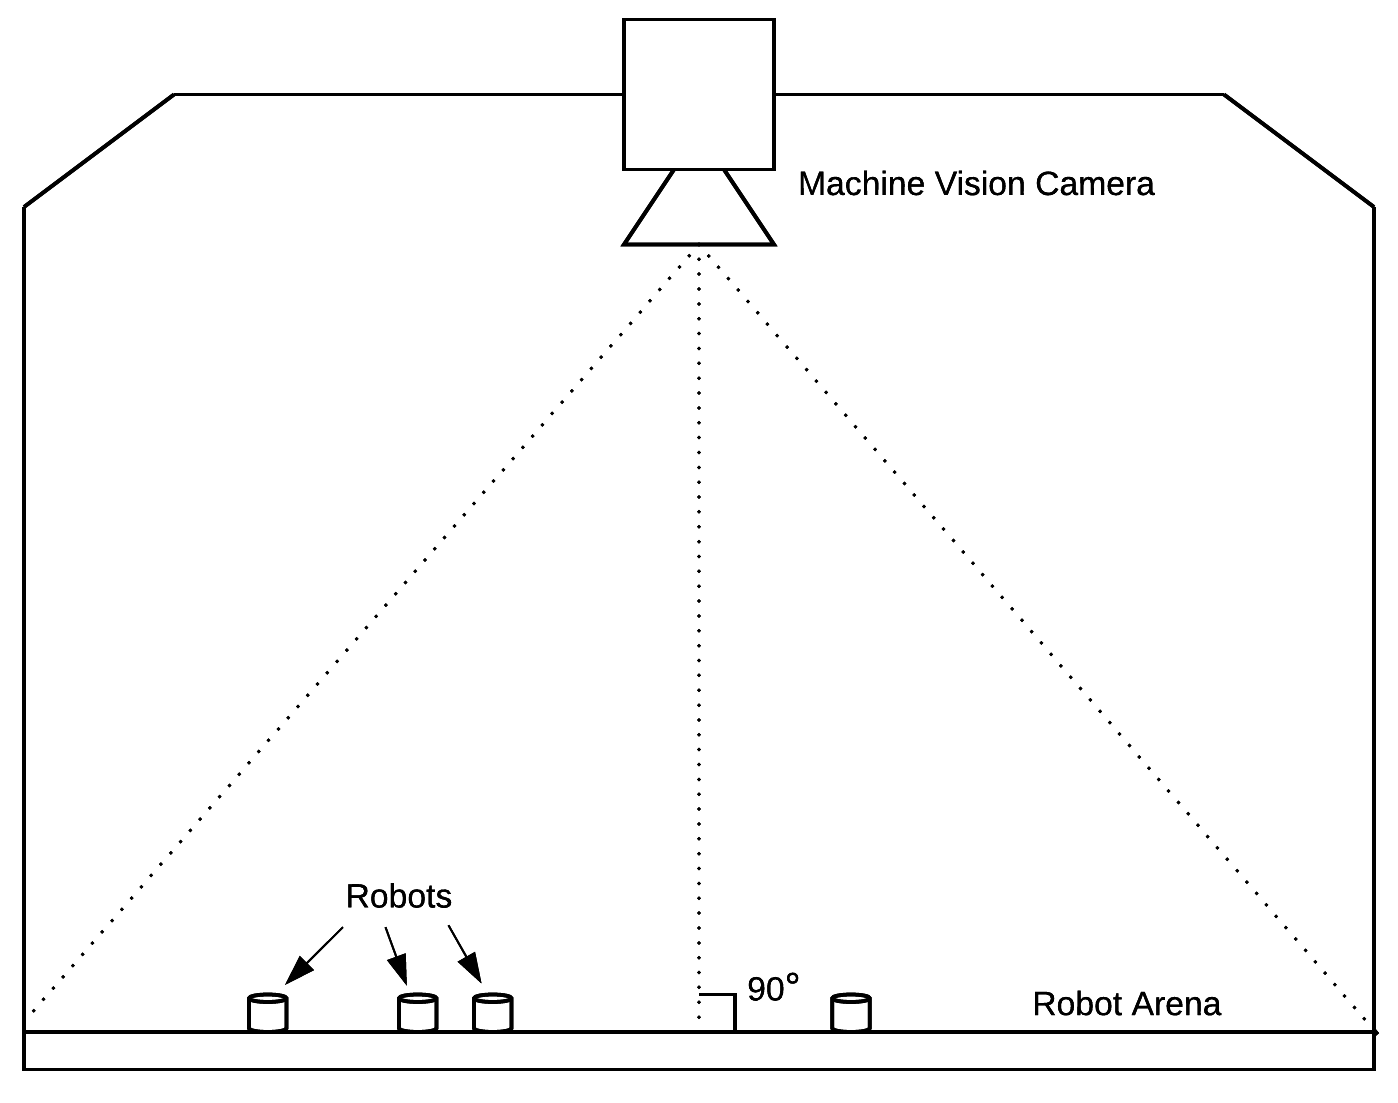
\includegraphics[scale=0.3]{Figures/CameraLayout.png}
	\decoRule
	\caption[Tracking Camera Arrangement]{Arrangement of the tracking camera over the robot arena.}
	\label{fig:CameraLayout}
\end{figure}

The image processing in these ongoing research efforts was performed using the `ARuCo\cite{Garrido:2014}' fiducial marker based tracking system, discussed further in section \ref{ARuCo}. It was determined that incorporating this existing infrastructure into this project would be the quickest way to achieve an operational tracking system, allowing work to focus on the novel aspects of this project sooner.

\begin{figure}
	\centering
	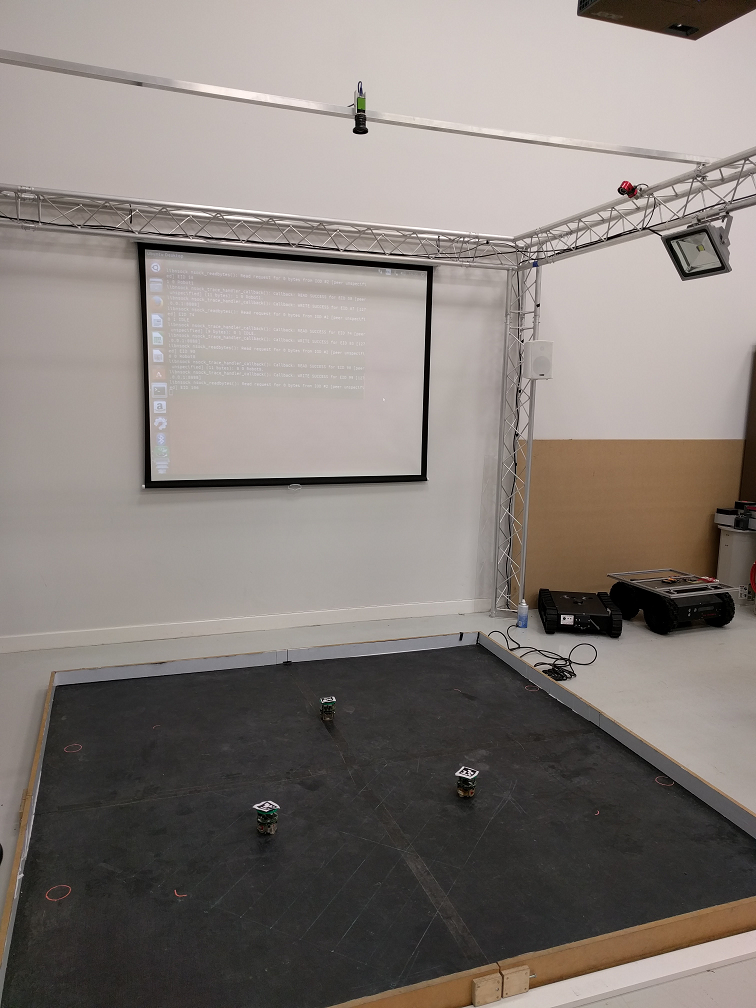
\includegraphics[scale=0.4]{Figures/ArenaPhoto.png}
	\decoRule
	\caption[Robot Arena and Tracking Camera]{The robot arena set up at the YRL, with tracking camera visible.}
	\label{fig:ArenaPhoto}
\end{figure}

%----------------------------------------------------------------------------------------

\section{Camera}
The camera used in the aforementioned tracking set-up is a JAI Go 5000C-PGE colour, area-scan camera, shown in figure \ref{fig:Camera}. It features a 1-inch, 5-megapixel CMOS sensor, with a maximum resolution of 2560 by 2048 pixels, capable of capturing 22 frames per second at full resolution, and up to 163.5 frames per second with reduced resolution and colour quality. The camera also features a global shutter, meaning it captures the full area of the image simultaneously, as opposed to a rolling shutter which captures portions of the image sequentially. This camera is well suited to marker tracking applications for a number of reasons. The high resolution means that even small markers, or markers that are relatively far from the camera will be captured with sufficient detail to be tracked and identified. The relatively high frame-rate means that the tracked positions can be recalculated regularly, and the video will appear smooth. The use of a global shutter avoids issues present in rolling shutter cameras, where a moving marker appears broken due to the time difference between the capture of two areas of the image and the movement of the marker during this time.

\begin{figure}
	\centering
	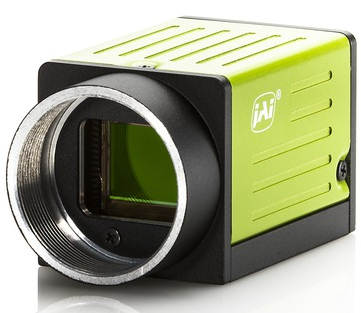
\includegraphics[scale=0.8]{Figures/Camera.png}
	\decoRule
	\caption[JAI-Go Camera]{The JAI-Go 5000C-PGE camera \cite{JAIGoCamera}.}
	\label{fig:Camera}
\end{figure}

The camera is connected to a server rack using Gigabit Ethernet cable, which is required to support the high bandwidth output of the camera due to its resolution and frame rate. This cable also provides power to the camera. A high resolution lens is fitted, with a relatively wide range of possible focal ratios from $f/1.4$ to $f/16$, allowing the camera to be adjusted to work well in a range of light conditions. With the lens included the camera has approximate dimensions of $29 \times 29 \times 100$ mm, and a weight of 246 grams, making it a very compact, lightweight solution.

The image data from the camera is transmitted in accordance with the `\textit{GigE Vision}' interface standard \cite{GigEVision}. This standard was first introduced in 2006, and is designed for transmitting video from high-performance industrial cameras over Ethernet networks. The `Common Vision Blox' (CVB) machine vision programming library is used to map the data from the GigE format to the OpenCV image format, so that it can be processed by an application.

%----------------------------------------------------------------------------------------

\section{ARuCo Tracking System} \label{ARuCo}
Developed by a team from the Computing and Numerical Analysis Department at Cordoba University in Spain, the ARuCo tag generation and detection system \cite{Garrido:2014} is a powerful fiducial marker creation and tracking tool. It comprises an algorithm for producing a `dictionary' of square, black and white, coded markers, and a method for automatically detecting these markers in a given image. These markers can be easily printed using a standard inkjet printer, and attached to surfaces and objects. Figure \ref{fig:ARuCoTags} shows four possible marker variations on standard printer paper. The stated applications for the ARuCo system include augmented reality, machine vision, and robot localisation. One of the main benefits of this system over other fiducial marker systems is the execution speed. By first using edge-detection methods to isolate the outlines of potential markers in the image, the system can eliminate a large portion of the image before applying the more complex processing to identify and differentiate individual markers \cite{Garrido:2014}. This makes the algorithm extremely efficient, and therefore makes it possible for the ARuCo system to be run in real time, even with relatively modest computational power. In a conventional use case the orientation of the camera can be calculated based on the positions of the corners of a marker, given that the marker's orientation is known. In this use case the reverse is true, the camera's position is fixed, and therefore the orientation of the robot can be determined based on the position and orientation of the corners of its marker, relative to the camera.

\begin{figure}
	\centering
	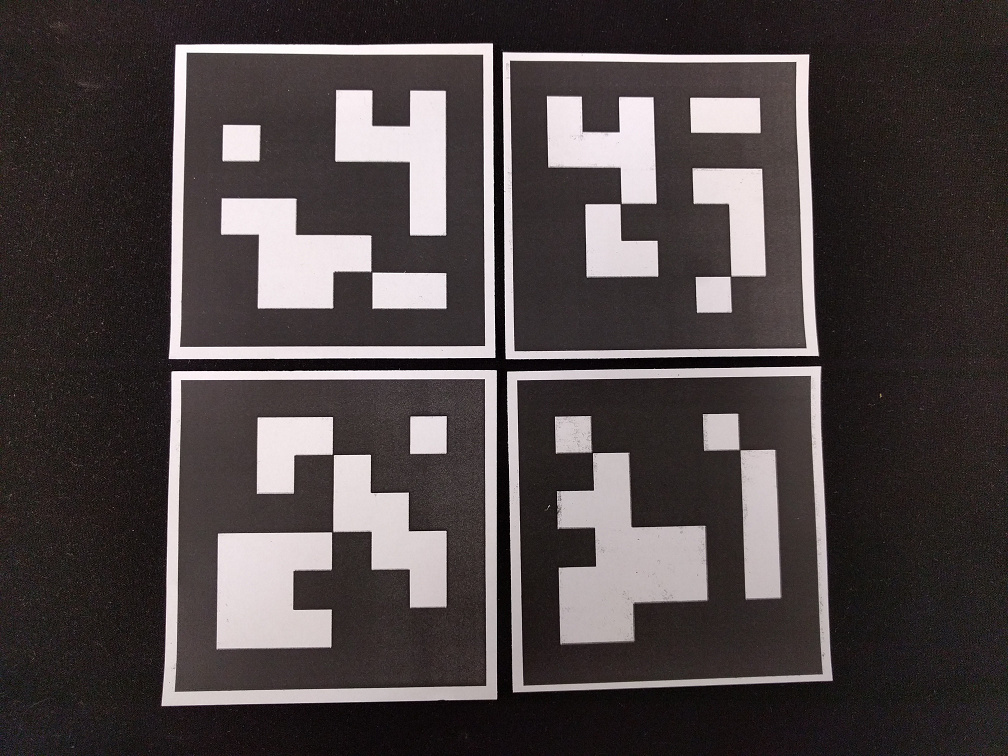
\includegraphics[scale=0.4]{Figures/ARuCoTags.png}
	\decoRule
	\caption[ARuCo Markers]{Four markers generated by the ARuCo fiducial marker generation and detection system.}
	\label{fig:ARuCoTags}
\end{figure}

Each of the e-puck robots used in this project were assigned an ID number, and a dictionary of ARuCo markers was generated to match. The markers were affixed to the top of the robots, oriented to match their forward directions. Figure \ref{fig:EPuckAruco} shows a laser printed ARuCo marker mounted on top of an e-puck robot. Some cursory preliminary tests of the tracking system confirmed that the markers could be accurately and reliably detected in the camera images, at a decent frame rate. Further detail of the integration of the ARuCo marker tracking system into the application developed during this project is given in section \ref{VideoFeedAndTrackingSystem}.

\begin{figure}
	\centering
	\includegraphics[scale=0.5]{Figures/EPuckARuCo.png}
	\decoRule
	\caption[ARuCo Marker Mounted on E-Puck]{A laser printed ARuCo marker mounted on top of an e-puck robot.}
	\label{fig:EPuckARuCo}
\end{figure}

%----------------------------------------------------------------------------------------